\section{Proses Instalasi}
Pembuatan sistem face detection dan face recognition akan menggunakan bahasa pemrograman Python dan \emph{library} openCV. 
Berikut adalah cara instalasi Python serta library openCV yang akan digunakan.

\subsection{Instalasi Python}
Instalator Python dapat didownload pada website resmi python \url{https://www.python.org/downloads}
\begin{figure}[h!]
    \centering
    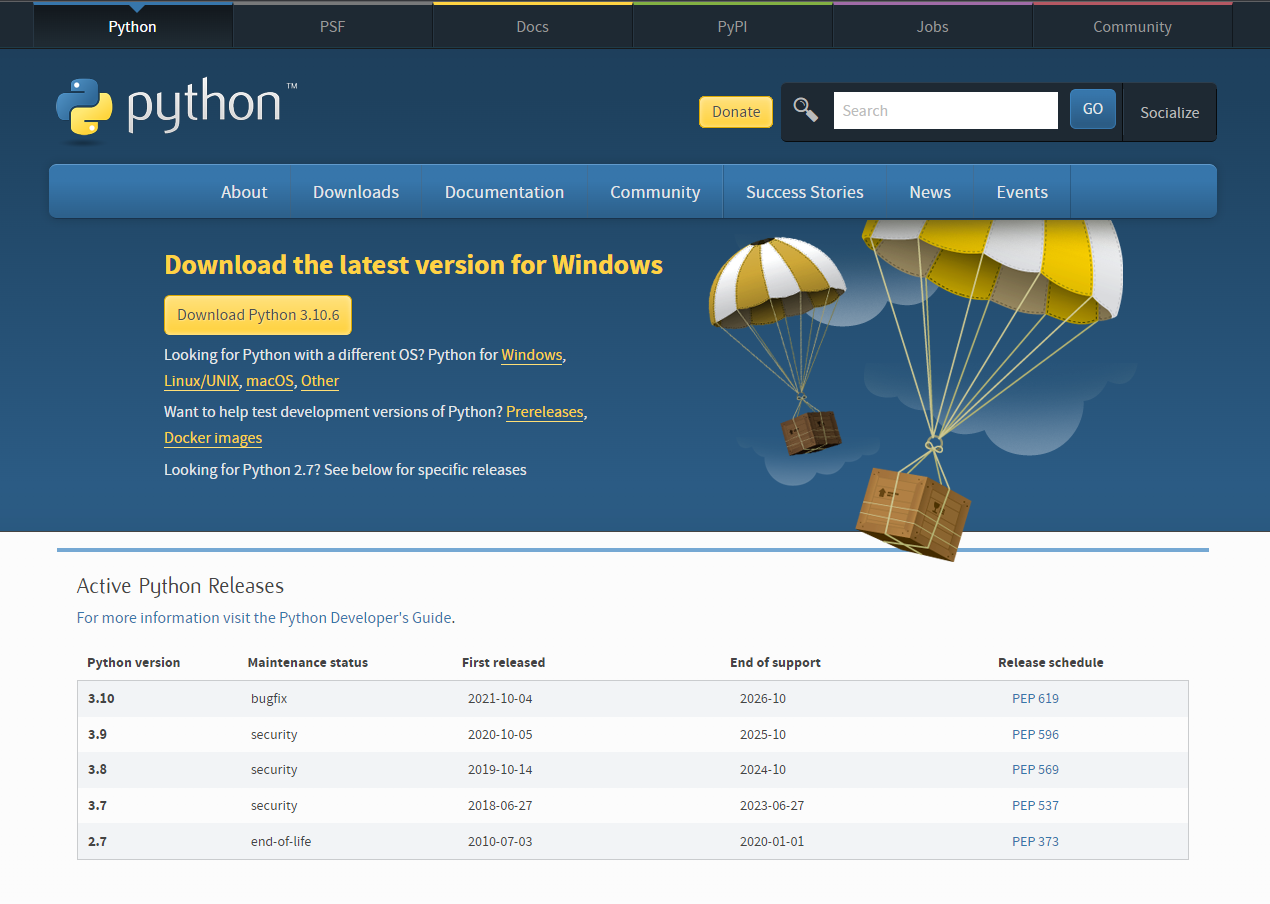
\includegraphics[width=0.9\linewidth]{images/web_py.PNG}
    \caption{Website resmi python}
\end{figure}
\\Download instalator versi terbaru dari python atau sesuaikan dengan kebutuhan penggunaan
\begin{figure}[h!]
    \centering
    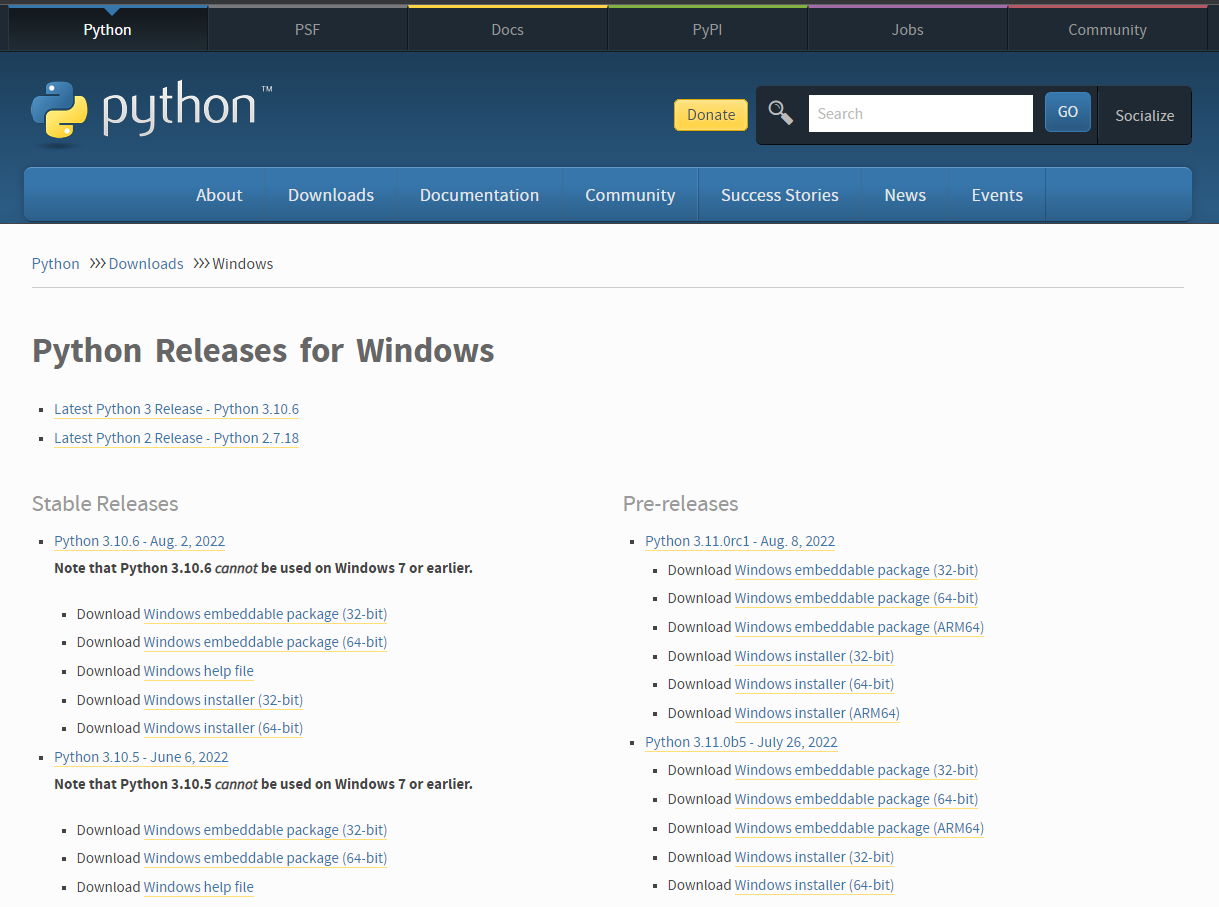
\includegraphics[width=0.9\linewidth]{images/py_ver.PNG}
    \caption{Pilihan Versi Python}
\end{figure}
\\Kemudian, buka file instalator python yang telah didownload, centang "Add Python 3.10 to PATH" dan klik \emph{Customize Installation}
\begin{figure}[h!]
    \centering
    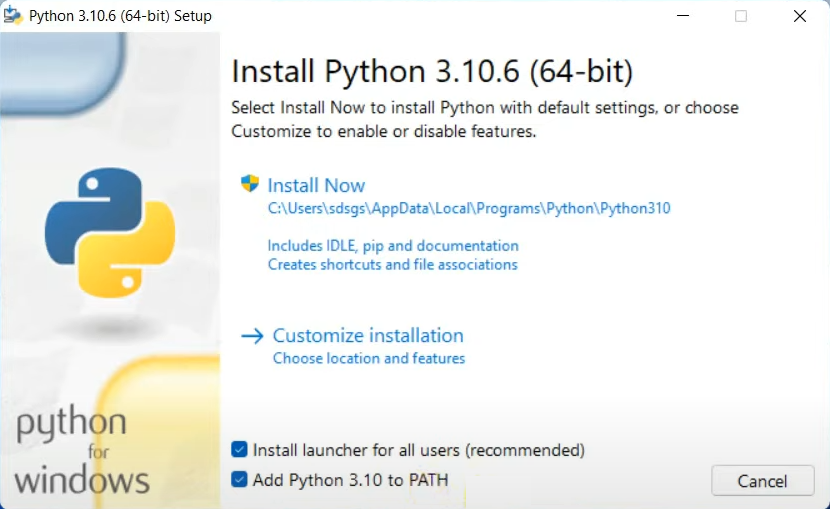
\includegraphics[width=0.9\linewidth]{images/py_1.PNG}
    \caption{Instalator python}
\end{figure}
\\Pilih fitur yang akan digunakan, untuk saran pilih semua fitur agar instalasi python lengkap, lalu klik 'next'
\begin{figure}[h!]
    \centering
    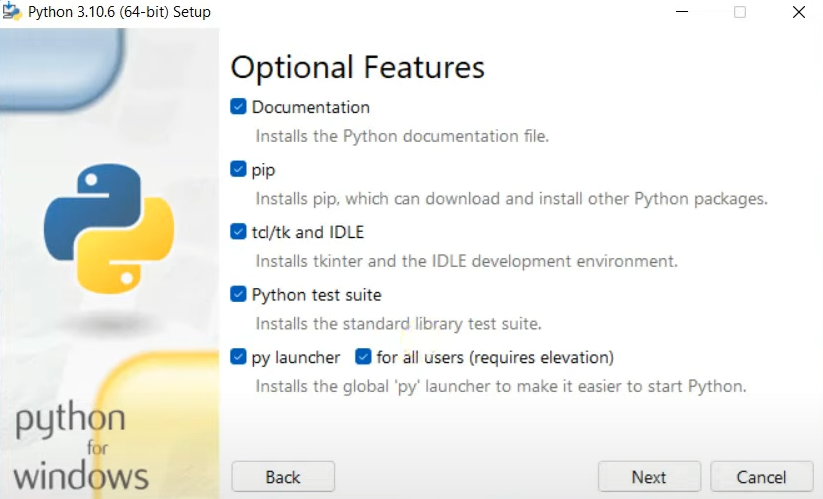
\includegraphics[width=0.9\linewidth]{images/py_2.PNG}
    \caption{Pilihan fitur}
\end{figure}
\\Centang pilihan sesuai pada gambar, kemudian pilih direktori untuk lokasi penyimpanan instalasi python sesuai kebutuhan. Lalu klik "Install" dan tunggu hingga proses instalasi selesai.
\begin{figure}[h!]
    \centering
    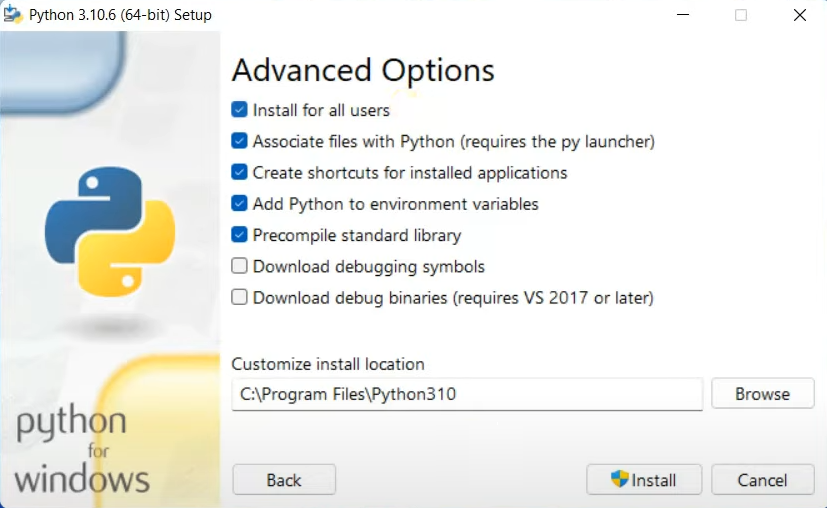
\includegraphics[width=0.9\linewidth]{images/py_3.PNG}
    \caption{Pilihan lanjutan dan penyesuaian lokasi}
\end{figure}

\subsection{Instalasi OpenCV}
Untuk Instalasi openCV dapat dilakukan melalui CMD(\emph{Command Prompt}). Buka direktori penyimpanan instalasi python, lalu menuju direktori 'Scripts' tempat pip.exe berada. Lalu tuliskan perintah \emph{pip install opencv-contrib-python} untuk memulai instalasi openCV, tunggu instalasi hingga selesai.
\begin{figure}[h!]
    \centering
    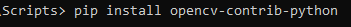
\includegraphics[width=0.7\linewidth]{images/opencv_1.PNG}
    \caption{Instalasi openCV}
\end{figure}
\\Setelah instalasi selesai, buka python IDLE atau pada CMD didalam direktori instalasi python, buka python.\\

Setelah python terbuka, ketik \textbf{import cv2} lalu enter, jika saat pengecekan openCV pada python tidak terjadi error, maka openCV berhasil di-install.
\begin{figure}[h!]
    \centering
    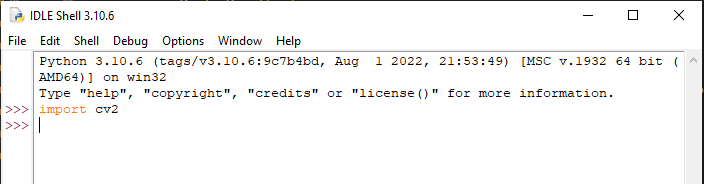
\includegraphics[width=1\linewidth]{images/opencv_2.PNG}
    \caption{Cek openCV pada python IDLE}
    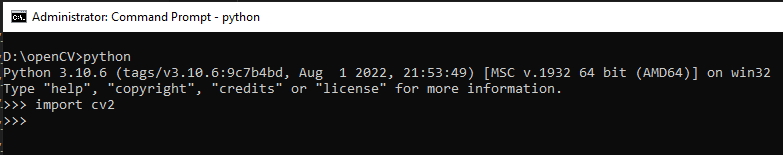
\includegraphics[width=1\linewidth]{images/opencv_3.PNG}
    \caption{Cek openCV pada CMD}
\end{figure}